\documentclass[14pt,t]{beamer}
\usepackage{fontspec}
\usepackage{color}
\usepackage{xcolor}
\usepackage{minted}
\usepackage{pgfplots}
\usepackage{etoolbox}
\usepackage[group-separator={'}]{siunitx}

%% These fonts are non-free.
%% Comment out the lines if you don't have them.
\setmainfont{Equity Text A}
\setsansfont{Concourse T3}
\setmonofont{Triplicate T4}

\definecolor{bgcolor}{RGB}{20,25,28}
\definecolor{codecolor}{RGB}{249,38,114}
\hypersetup{colorlinks,linkcolor=,urlcolor=codecolor}
\setbeamercolor{background canvas}{bg=bgcolor}
\setbeamercolor{normal text}{fg=white}
\setbeamercolor{itemize item}{fg=lightgray}
\setbeamercolor{itemize subitem}{fg=lightgray}
\setbeamercolor{itemize subsubitem}{fg=lightgray}
\setbeamercolor{enumerate item}{fg=lightgray}
\setbeamercolor{page number in head/foot}{fg=lightgray}
\setbeamerfont{page number in head/foot}{size=\large}
\setbeamertemplate{itemize items}[circle]
\setbeamertemplate{navigation symbols}{}
\setbeamertemplate{footline}{
  \hfill%
  \usebeamercolor[fg]{page number in head/foot}%
  \usebeamerfont{page number in head/foot}%
  \setbeamertemplate{page number in head/foot}[framenumber]%
  \usebeamertemplate*{page number in head/foot}\kern1em\vskip2pt%
}

\usemintedstyle{monokai}
\newminted[rustcode]{rust}{fontsize=\footnotesize}
\renewcommand{\footnotesize}{\tiny}

\def\code#1{{\color{codecolor}\texttt{#1}}}

\renewcommand{\theFancyVerbLine}{\color{darkgray}\large \oldstylenums{\arabic{FancyVerbLine}}}
\renewcommand{\title}[1]{
  {\huge #1} \vskip 0.4cm
}
\renewcommand{\subtitle}[1]{
  \vskip 0.3cm {\Large #1} \vskip 0.2cm %
}

\usetikzlibrary{
  pgfplots.colorbrewer,
}
\pgfplotsset{
  % define a `cycle list' for marker
  cycle list/.define={my marks}{
    every mark/.append style={solid,fill=\pgfkeysvalueof{/pgfplots/mark list fill}},mark=*\\
    every mark/.append style={solid,fill=\pgfkeysvalueof{/pgfplots/mark list fill}},mark=square*\\
    every mark/.append style={solid,fill=\pgfkeysvalueof{/pgfplots/mark list fill}},mark=triangle*\\
    every mark/.append style={solid,fill=\pgfkeysvalueof{/pgfplots/mark list fill}},mark=diamond*\\
  },
}

\pgfplotsset{tikzDefaults/.style=
  {legend pos=outer north east,
    legend style={fill=none},
    ymajorgrids=true,
    grid style=dashed,
    cycle list/Spectral-11,
    cycle multiindex* list={
      Spectral-11
      \nextlist
      my marks
      \nextlist
      [3 of]linestyles
      \nextlist
      very thick
      \nextlist},
  }}

\makeatletter
\newcommand{\latencyplot}[3]{%
  \begin{tikzpicture}
    \begin{axis}[
      tikzDefaults,
      title={Median Latency (#1 workers)},
      ylabel={Epoch Size [n]},
      xlabel={Epoch Latency [s]},
      xmode=log, ymode=log,
      x tick label style={/pgf/number format/fixed},
      ]
      
      \forcsvlist{\latencyplot@item{#1}}{#2}
      \ifthenelse{ \equal{#3}{} }{}{\legend{#3}}
    \end{axis}
  \end{tikzpicture}}

\newcommand{\latencyplot@item}[2]{%
  \addplot table[y index=0, x index=#2] {../data/latency-#1.csv};%
}

\newcommand{\scalingplot}[3]{%
  \begin{tikzpicture}
    \begin{axis}[
      tikzDefaults,
      title={Scaling (\num{#1} events/epoch)},
      xlabel={Workers [n]},
      ylabel={Epoch Latency [s]},
      xmode=log,
      log basis x={2},
      scaled y ticks=false,
      y tick label style={/pgf/number format/fixed},
      xtick={1, 2, 4, 8, 16, 32},
      ]
      
      \forcsvlist{\scalingplot@item{#1}}{#2}
      \ifthenelse{ \equal{#3}{} }{}{\legend{#3}}
    \end{axis}
  \end{tikzpicture}}

\newcommand{\scalingplot@item}[2]{%
  \addplot table[x index=0, y index=#2] {../data/scaling-#1.csv};%
}

\newcommand{\cdfplot}[4]{%
  \begin{tikzpicture}
    \begin{axis}[
      tikzDefaults,
      title={CDF (#1 workers, \num{#2} events/epoch)},
      xlabel={Epoch Latency [s]},
      ylabel={CDF [\%]},
      xmode=log,
      ]
      
      \forcsvlist{\cdfplot@item{#1}{#2}}{#3}
      \ifthenelse{ \equal{#4}{} }{}{\legend{#4}}
    \end{axis}
  \end{tikzpicture}}

\newcommand{\cdfplot@item}[3]{%
  \addplot table[skip first n=1, y index=0, x index=#3] {../data/cdf-#1-#2.csv};%
}

\makeatother

\begin{document}
\begin{frame}[b,plain]
  \begin{center}
    {\LARGE Implementation of a Benchmark Suite for Strymon} \\
    \vspace{0.5cm}
    Nicolas Hafner \\
    \vfill
    \hspace*{-1cm}\begin{minipage}{\pagewidth}
      \begin{center}
        \hspace{0.5cm}
        
\includegraphics[height=1cm]{../systems-cover/ethlogo_white.pdf}
        \hfill
        
\includegraphics[height=1cm]{../systems-cover/inf-logo_white.pdf}
        \hfill
        
\includegraphics[height=1cm]{../systems-cover/systemslogo-3colour_white.pdf}
        \hspace*{0.5cm}
      \end{center}
    \end{minipage} 
  \end{center}
\end{frame}

\begin{frame}
  \makebox[\linewidth][c]{
    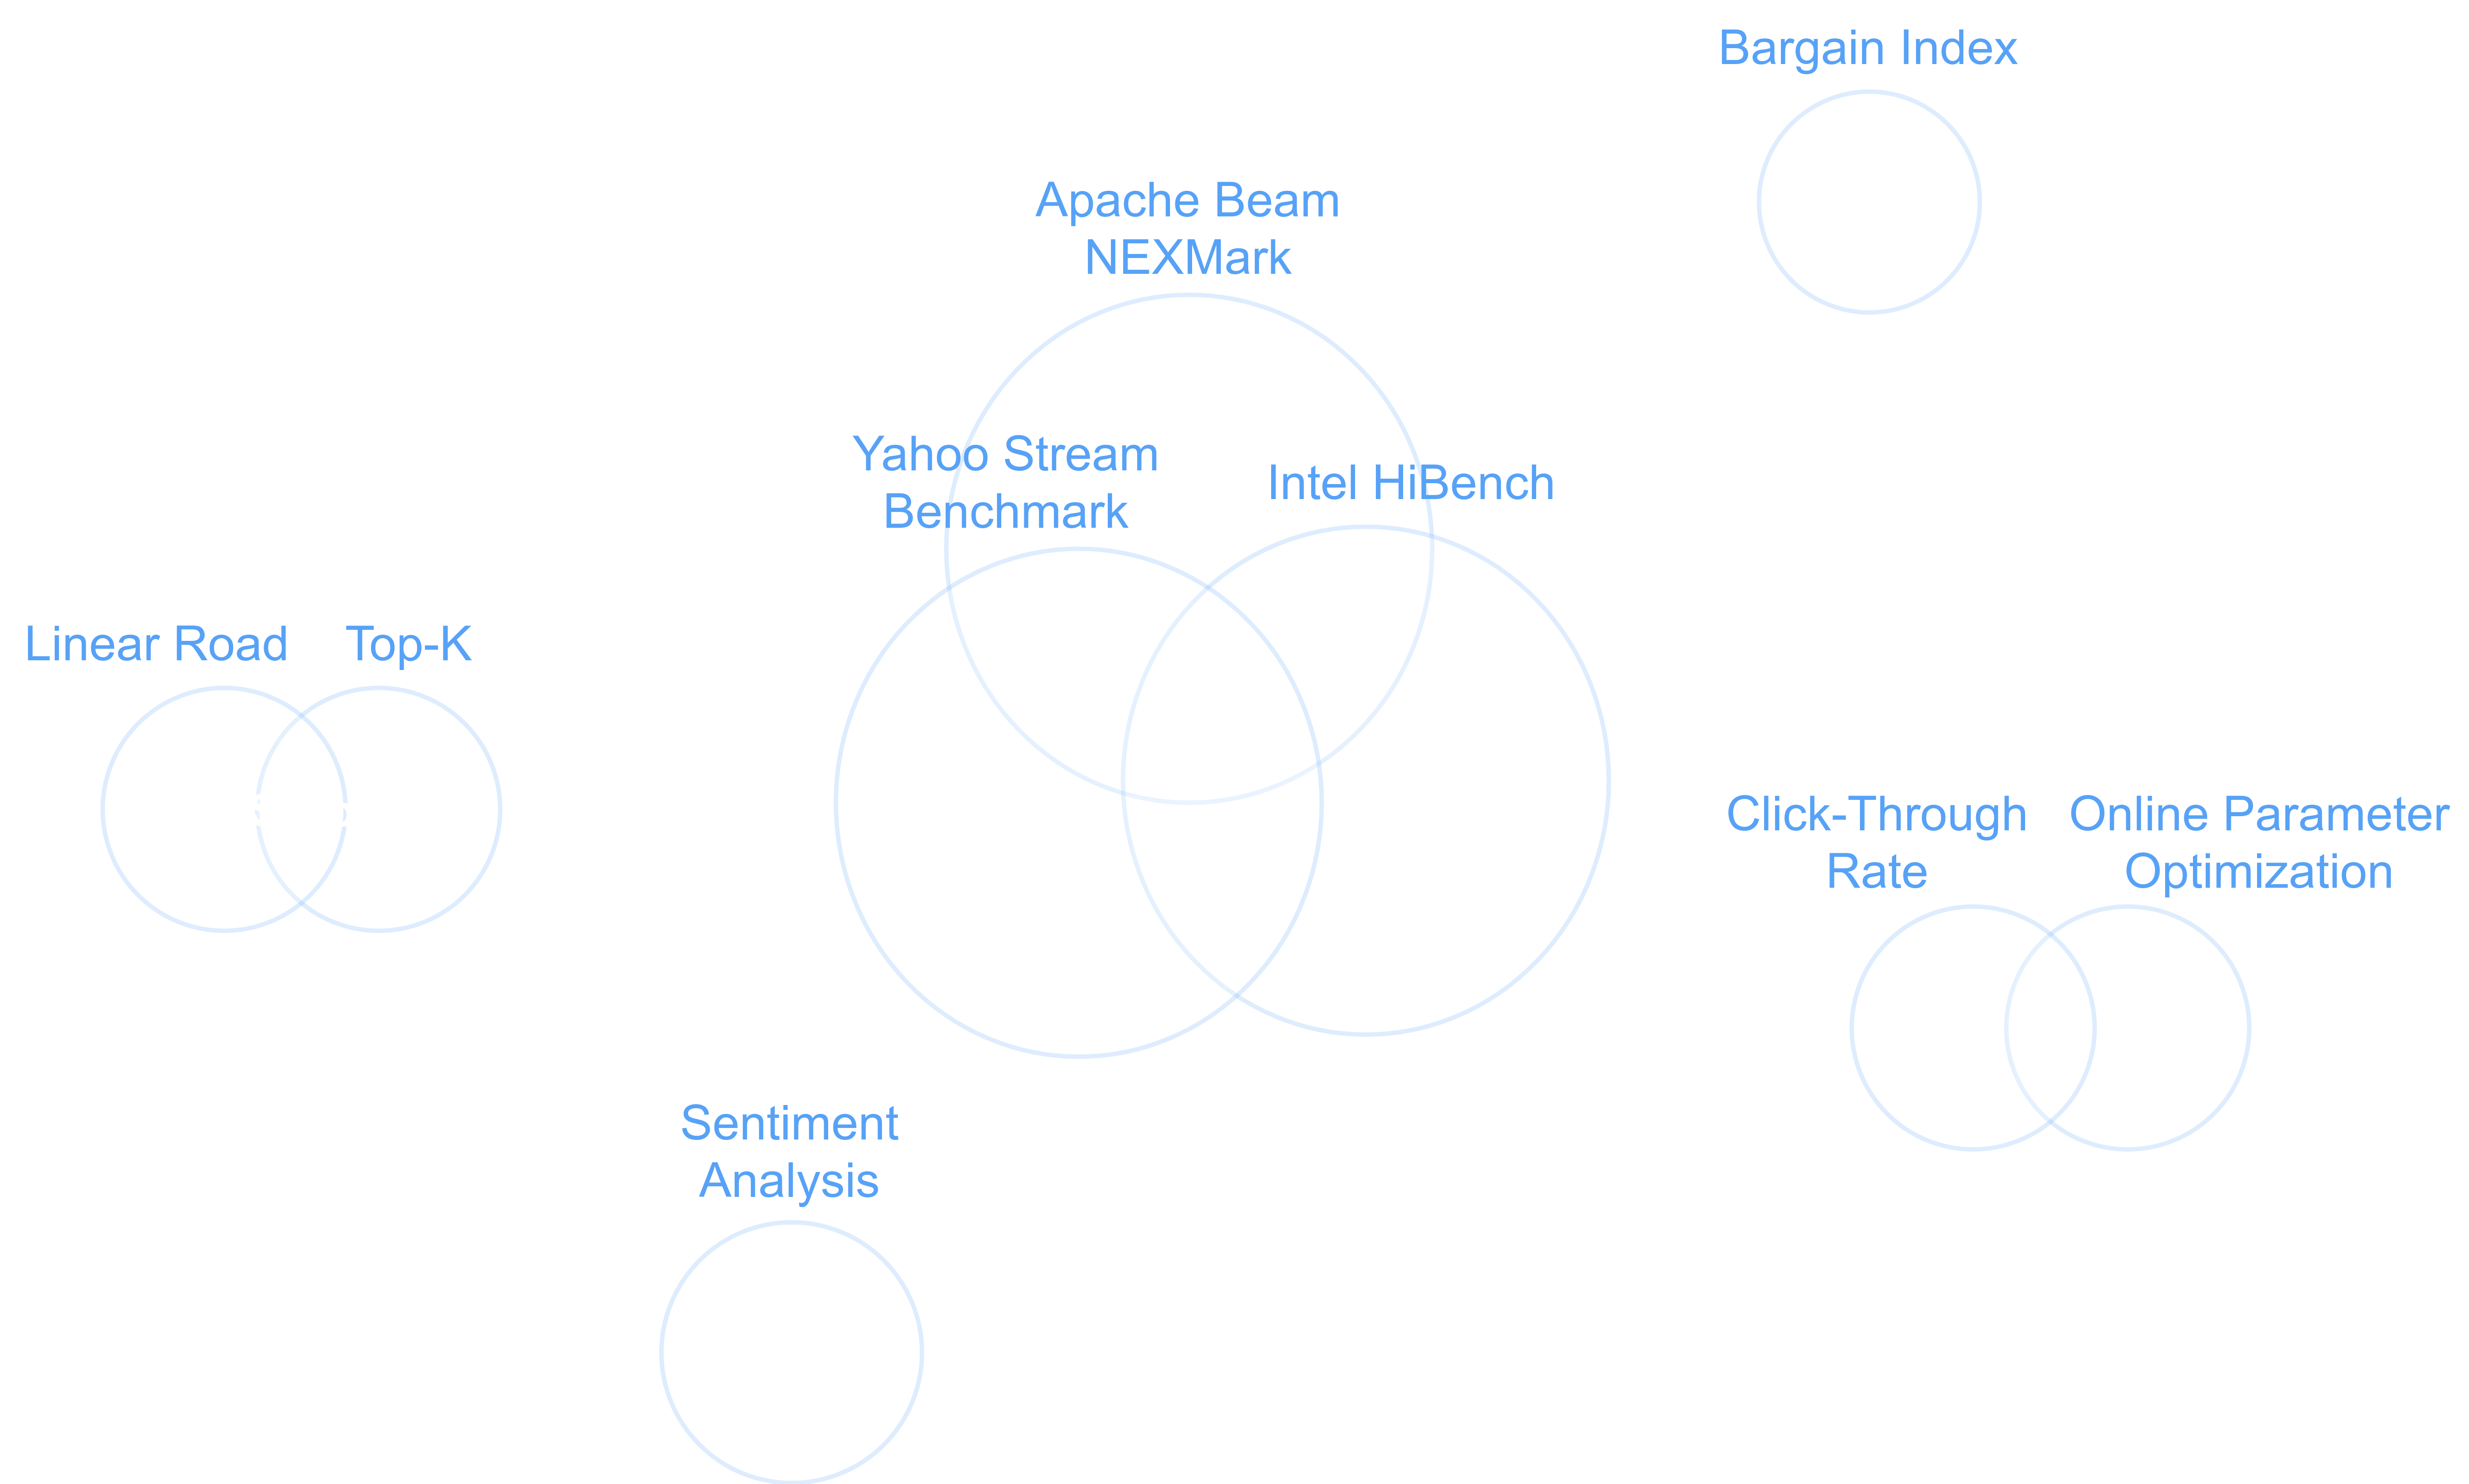
\includegraphics[width=\pagewidth]{benchmarks.png}
  }
\end{frame}

\begin{frame}
  \title{Current Publications}
  \begin{itemize}
  \item Investigated current practises in published papers
  \item Almost no paper used a standardised benchmark
  \item Code and data often not published
  \item Often very simple benchmarks like Word Count:
  \end{itemize}
  \vspace{1cm}
  \begin{center}
    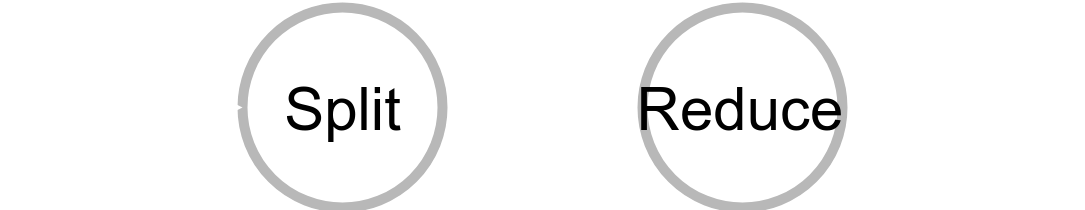
\includegraphics[height=0.75cm]{hib-3.png}
  \end{center}
\end{frame}

\begin{frame}
  \title{Timely}
  \begin{center}
    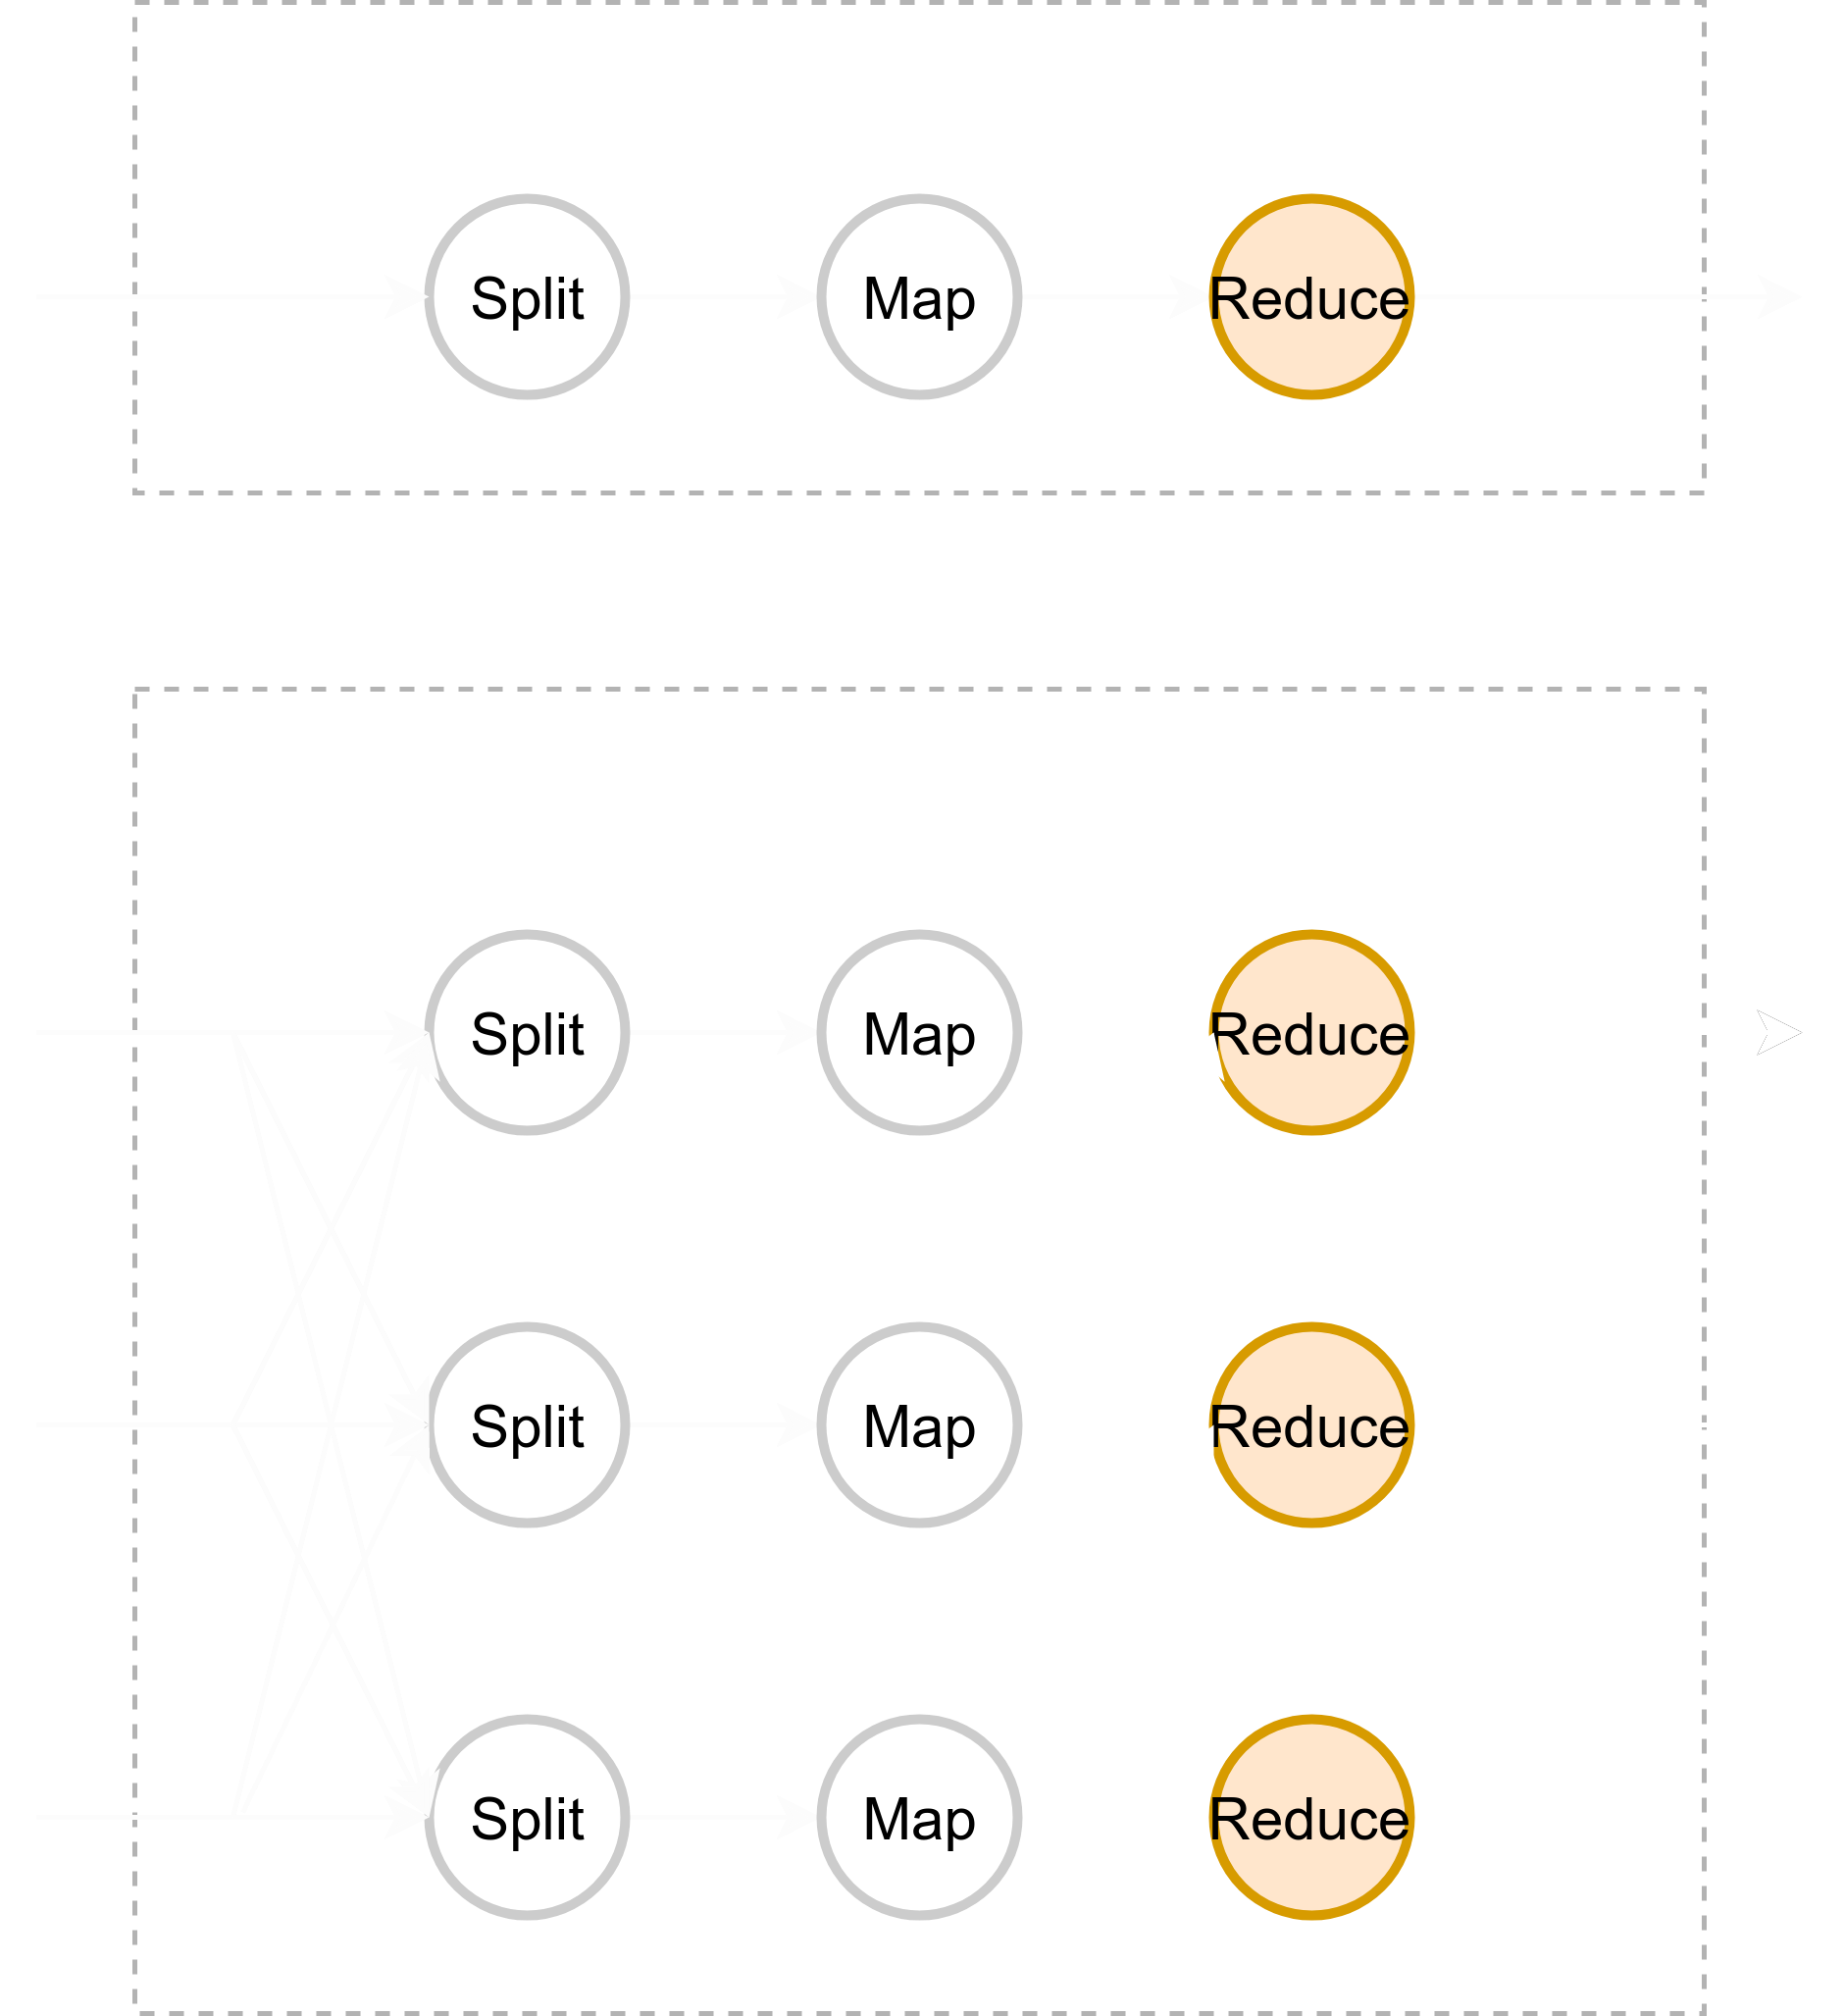
\includegraphics[height=8cm]{dataflow.png}
  \end{center}
\end{frame}

\begin{frame}
  \title{Timely}
  \vspace*{2cm}
  \begin{center}
    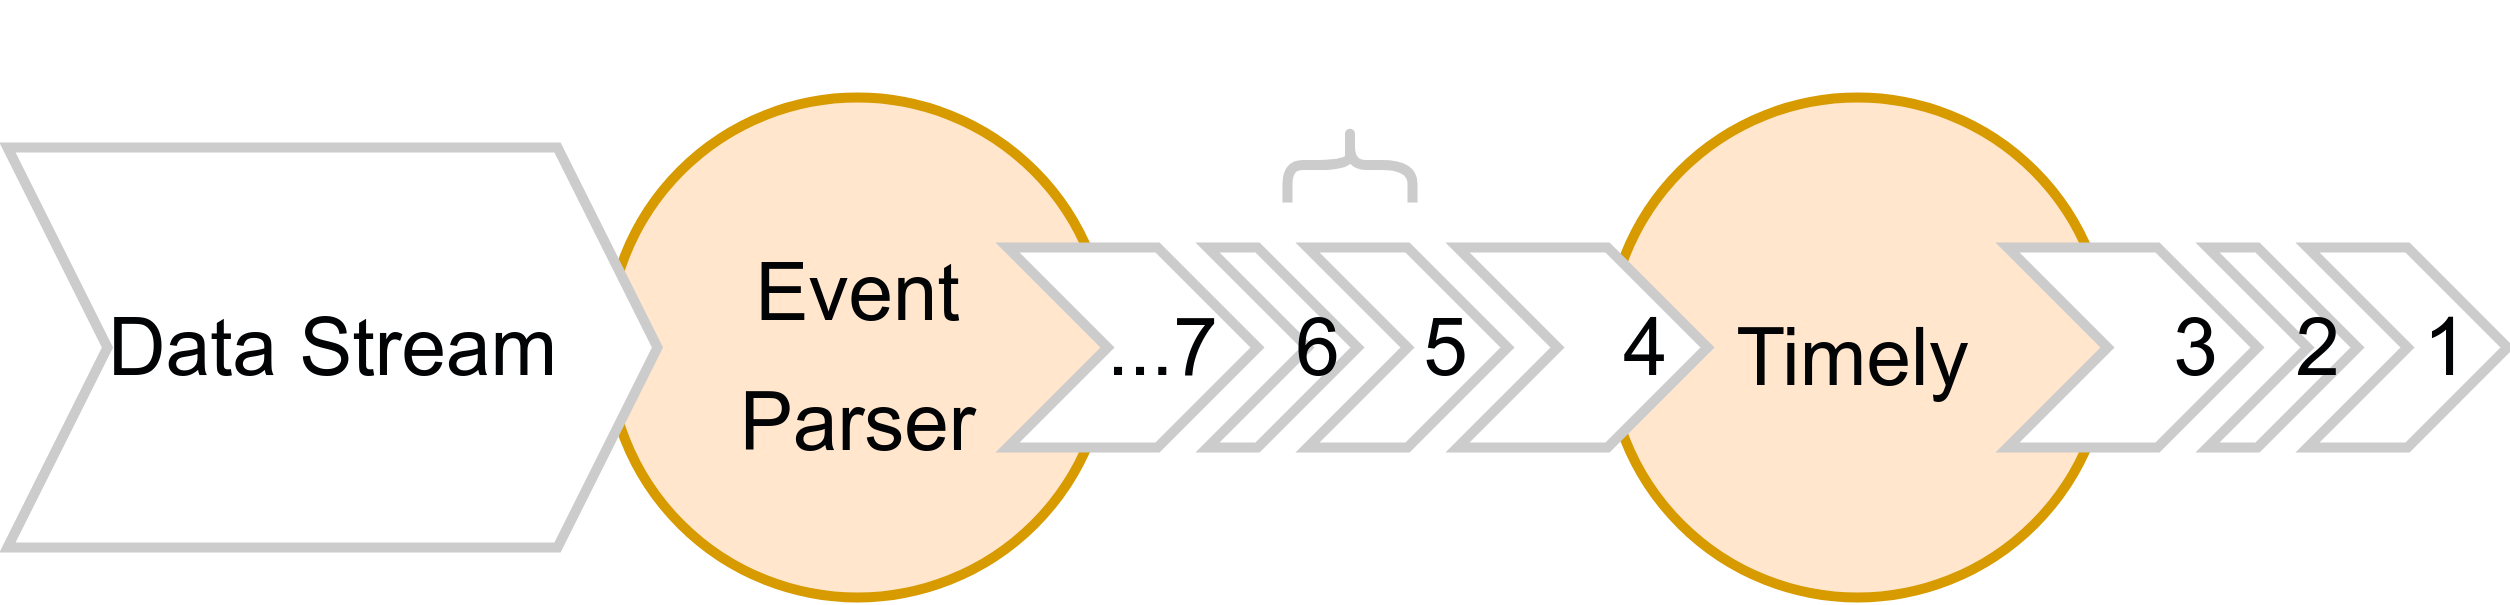
\includegraphics[height=2cm]{epochs.png}
  \end{center}
\end{frame}

\begin{frame}
  \title{Benchmarks}
  \begin{itemize}
  \item We implemented three benchmarks:
  \end{itemize}
  \begin{enumerate}
  \item Intel's HiBench
  \item Yahoo's Streaming Benchmark
  \item Apache Beam's NEXMark
  \end{enumerate}
  \begin{itemize}
  \item Comparable against many other systems
  \end{itemize}
\end{frame}

\begin{frame}
  \title{Intel's HiBench\footnotemark}
  \begin{itemize}
  \item Big Data micro-benchmark
  \item Only four data flows:
  \end{itemize}
  \begin{enumerate}
  \item Identity \hfill\raisebox{-.2\height}{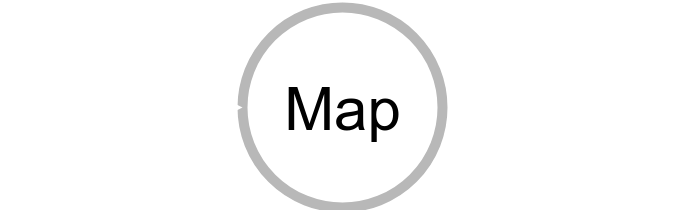
\includegraphics[height=0.75cm]{hib-1.png}}
  \item Repartition \hfill\raisebox{-.2\height}{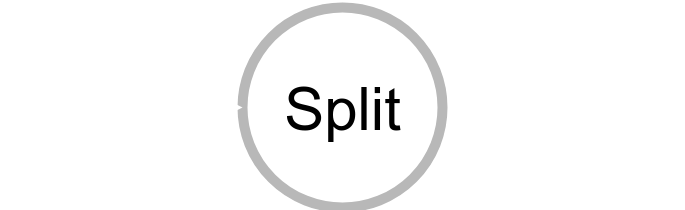
\includegraphics[height=0.75cm]{hib-2.png}}
  \item Word Count \hfill\raisebox{-.2\height}{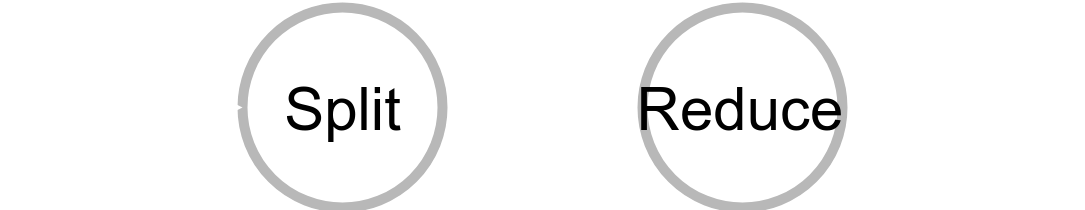
\includegraphics[height=0.75cm]{hib-3.png}}
  \item Window Reduce \hfill\raisebox{-.2\height}{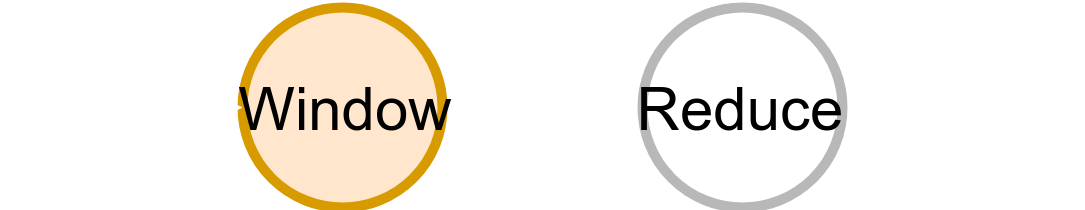
\includegraphics[height=0.75cm]{hib-4.png}}
  \end{enumerate}
  \footnotetext{\url{https://github.com/intel-hadoop/HiBench}}
\end{frame}

\begin{frame}
  \title{Yahoo Stream Benchmark\footnotemark}
  \begin{itemize}
  \item Count ad views for ad campaigns
  \item Only one, relatively simple data flow:
  \end{itemize}
  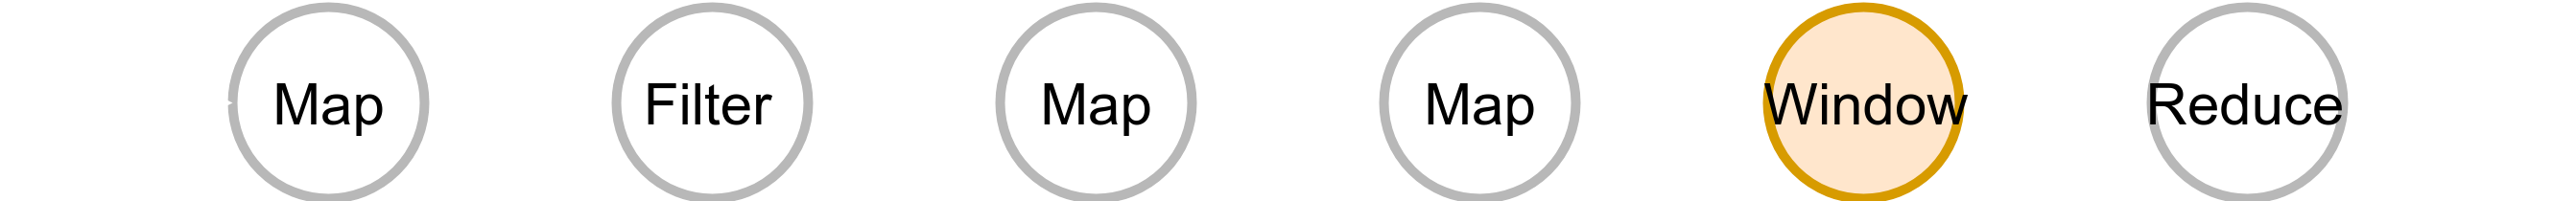
\includegraphics[height=0.75cm]{ysb.png}
  \footnotetext{Sanket Chintapalli et al. “Benchmarking streaming computation engines: Storm, Flink and Spark streaming”. In: Parallel and Distributed Processing Symposium Workshops, 2016 IEEE International. IEEE. 2016, pp. 1789–1792.}
\end{frame}

\begin{frame}
  \title{Beam's NEXMark\footnotemark}
  \begin{itemize}
  \item Implements an ``auctioning system''
  \item 13 data flows in total
  \item Uses filter, map, reduce, join, window, session, partition
  \item Dataflows for Query 5 and 8:
  \end{itemize}
  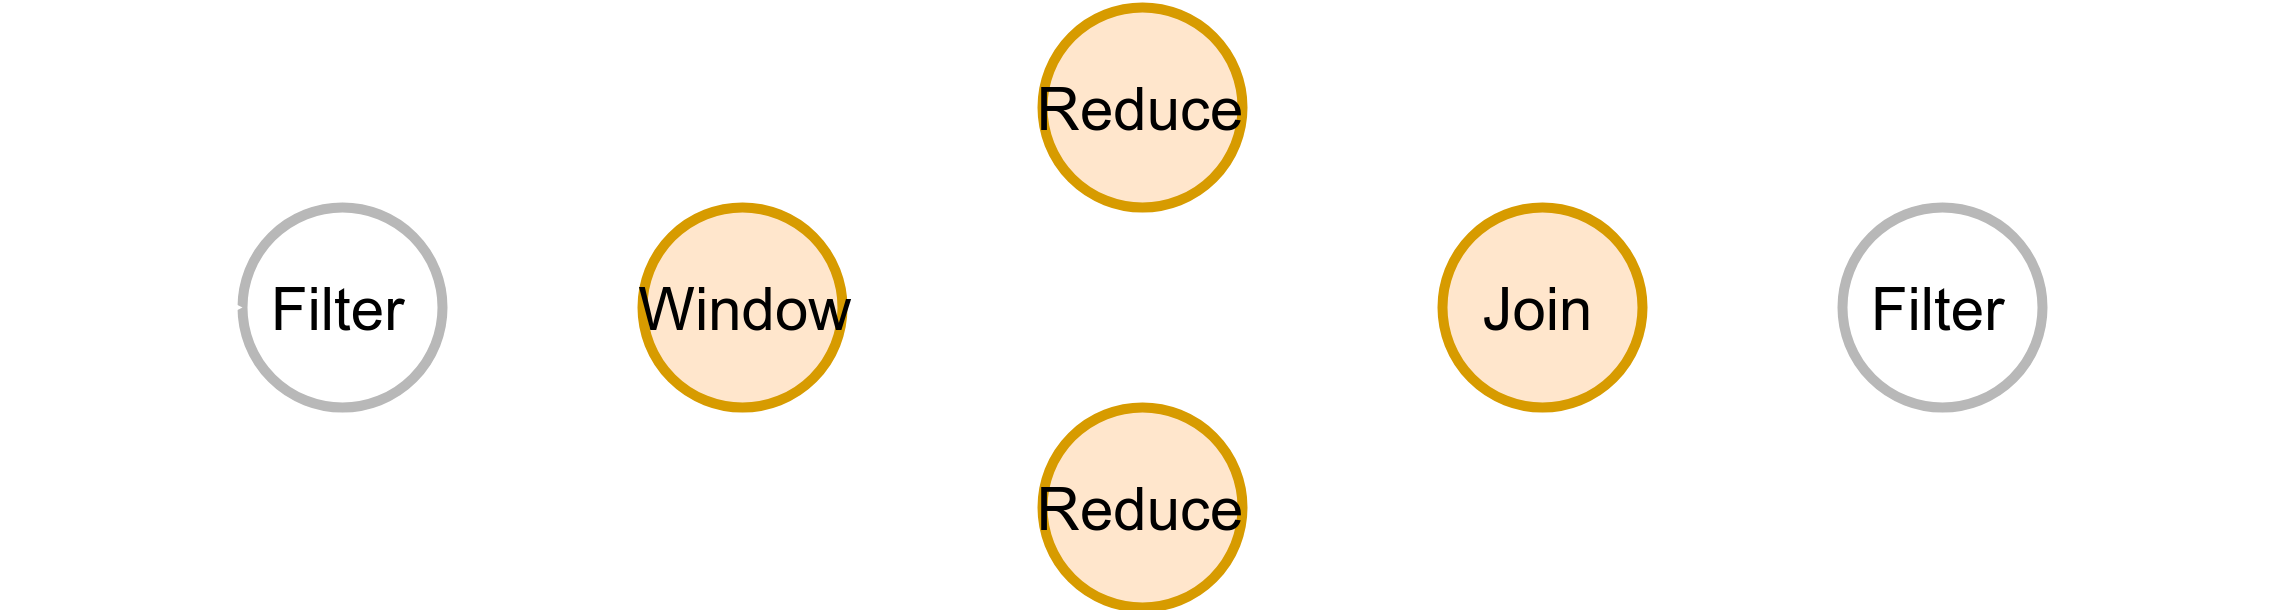
\includegraphics[height=1.5cm]{nex-5.png}
  \hfill
  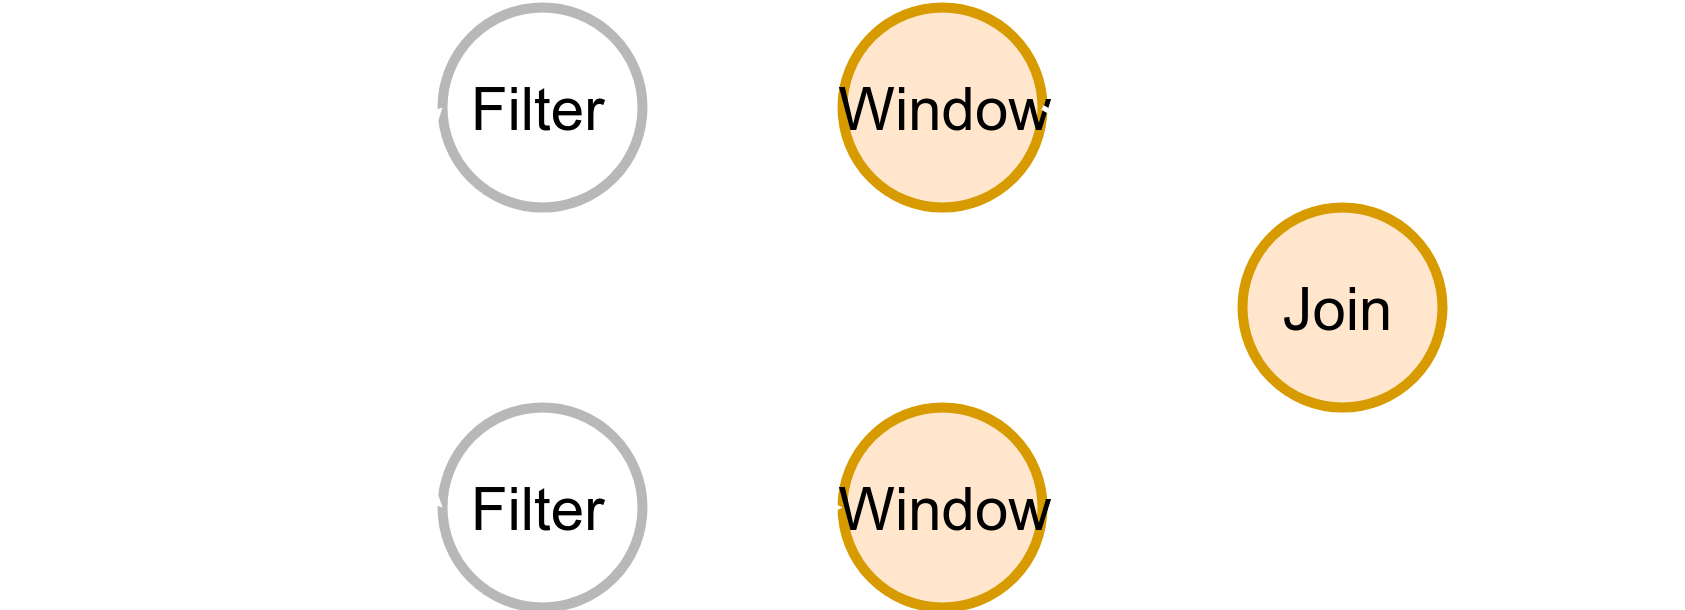
\includegraphics[height=1.5cm]{nex-8.png}
  \footnotetext{Based on original paper: Pete Tucker et al. NEXMark–A Benchmark for Queries over Data Streams (DRAFT). Tech. rep. Technical report, OGI School of Science \& Engineering at OHSU, Septembers, 2008.}
\end{frame}

\begin{frame}
  \title{Testing Framework}
  \begin{itemize}
  \item Implemented a general framework for benchmarks
  \item Generic components for input/output handling
  \item New, reusable operators for join, window, reduce, filtermap, session, partition
  \item Implemented HiBench, YSB, NEXmark using this framework
  \end{itemize}
\end{frame}

\begin{frame}
  \title{Evaluation System}
  \begin{itemize}
  \item Run on sgs-r815-03 (AMD, 64 cores, 2.4GHz)
  \item Data generated directly in memory
  \item Generation re-implemented in Rust
  \item No foreign systems like Kafka used
  \end{itemize}
\end{frame}

\begin{frame}
  \title{Evaluation Setup}
  \begin{itemize}
  \item Measured closed-loop per-epoch latency
  \item One epoch encompasses a logical second of data
  \item Workload varied between 1K-10Me/s, 1-32 workers, 10-120s windows
  \end{itemize}
\end{frame}

\begin{frame}
  \title{HiBench Latency / Batch}
  \latencyplot{32}{1,2,3,4}{Identity, Repartition, Wordcount, Fixwindow}
\end{frame}

\begin{frame}
  \title{HiBench CDF}
  \cdfplot{32}{10000000}{1,2,3,4}{Identity, Repartition, Wordcount, Fixwindow}
\end{frame}

\begin{frame}
  \title{YSB Latency / Batch}
  \latencyplot{32}{5}{}
\end{frame}

\begin{frame}
  \title{YSB CDF}
  \cdfplot{32}{10000000}{5}{}
\end{frame}

\begin{frame}
  \title{NEXMark Latency / Batch}
  \latencyplot{32}{6,7,8,9,10,11,12,13,14,15,16}{Q0, Q1, Q2, Q3, Q4, Q5, Q6, Q7, Q8, Q9, Q11}
\end{frame}

\begin{frame}
  \title{NEXMark CDF}
  \cdfplot{32}{10000000}{6,7,8,9,10,11,12,13,14,15,16}{Q0, Q1, Q2, Q3, Q4, Q5, Q6, Q7, Q8, Q9, Q11}
\end{frame}

\begin{frame}
  \title{Benchmark Evaluation}
  \begin{itemize}
  \item Benchmarks are underspecified and undocumented
    \pause
  \item No result verification
    \pause
  \item External systems compound complexity
    \pause
  \item No tests for load balancing, fault-tolerance, etc.
  \end{itemize}
\end{frame}

\begin{frame}
  \title{Benchmark Suggestions}
  \begin{itemize}
  \item Abstract model definitions for data flows
  \item Correctness verification tools
  \item Deterministically generated workloads
  \item Various short and long data flows
  \item Tests for both latency, \textit{and} fault-tolerance, etc.
  \end{itemize}
\end{frame}

\begin{frame}
  \vspace*{1cm}
  \scalebox{0.5}{
    \latencyplot{32}{6,7,8,9,10,11,12,13,14,15,16}{Q0, Q1, Q2, Q3, Q4, Q5, Q6, Q7, Q8, Q9, Q11}}
  \scalebox{0.5}{
    \cdfplot{32}{10000000}{6,7,8,9,10,11,12,13,14,15,16}{Q0, Q1, Q2, Q3, Q4, Q5, Q6, Q7, Q8, Q9, Q11}}
  \vspace*{0.1cm}
  \begin{center}
    \small
    \url{http://strymon.systems.ethz.ch/} \\
    \vspace*{0.3cm}
    \url{https://github.com/Shinmera/bsc-thesis}
  \end{center}
\end{frame}


%%%%%%%%%%%%%%%%%%%
%% BACKUP SLIDES %%
%%%%%%%%%%%%%%%%%%%

\begin{frame}
  \title{HiBench Worker Scaling}
  \scalingplot{10000000}{1,2,3,4}{Identity, Repartition, Wordcount, Fixwindow}
\end{frame}

\begin{frame}
  \title{YSB Worker Scaling}
  \scalingplot{10000000}{5}{}
\end{frame}

\begin{frame}
  \title{NEXMark Worker Scaling}
  \scalingplot{10000000}{6,7,8,9,10,11,12,13,14,15,16}{Q0, Q1, Q2, Q3, Q4, Q5, Q6, Q7, Q8, Q9, Q11}
\end{frame}

\begin{frame}
  \title{NEXMark Window Scaling}
  \begin{tikzpicture}
    \begin{axis}[
      tikzDefaults,
      title={Windowing (32 workers, \num{10000000} e/s)},
      xlabel={Window Size [n]},
      ylabel={Epoch Latency [s]},
      ]
      
      \addplot table[x index=0, y index=1] {../data/window-32-10000000.csv};
      \addplot table[x index=0, y index=2] {../data/window-32-10000000.csv};
      \legend{Q7,Q8}
    \end{axis}
  \end{tikzpicture}
\end{frame}

\begin{frame}
  \title{NEXMark Slide Scaling}
  \begin{tikzpicture}
    \begin{axis}[
      tikzDefaults,
      title={Window Slides Q5 (32 workers, \num{10000000} e/s)},
      xlabel={Window Size [n]},
      ylabel={Epoch Latency [s]},
      ]
      
      \addplot table[x index=0, y index=1] {../data/slide-32-10000000.csv};
      \addplot table[x index=0, y index=2] {../data/slide-32-10000000.csv};
      \addplot table[x index=0, y index=3] {../data/slide-32-10000000.csv};
      \addplot table[x index=0, y index=4] {../data/slide-32-10000000.csv};
      \addplot table[x index=0, y index=5] {../data/slide-32-10000000.csv};
      \legend{5s, 10s, 20s, 40s, 60s}
    \end{axis}
  \end{tikzpicture}
\end{frame}

\end{document}

%%% Local Variables:
%%% mode: latex
%%% TeX-master: t
%%% TeX-engine: luatex
%%% TeX-command-extra-options: "-shell-escape"
%%% End:
